\section{\cluethreed{} performance for displaced photons}
\label{sec:singlephoton}

The central question of this project is whether \cluethreed{} can reconstruct
a photon shower whose trajectory does not point back to the interaction
point. The displaced-photon study shows both a performance loss
and an unexpected structure: the loss develops in two stages, separated by a
plateau. The study shows that fragmentation induced by the origin-based
projection is the mechanism behind the observed loss.

\subsection{The performance loss is not a smooth decline}

We used single displaced photons without pileup, with Run4D121\footnote{The
CMSSW identifier for the specific Phase-2 detector geometry used in this
study.}
geometry and the default HLT \cluethreed{} configuration. The wide-range
production samples $\R$ uniformly from \SI{0}{cm} to \SI{350}{cm} and photon
energy from \SI{10}{GeV} to \SI{250}{GeV}, subject to the front and
back HGCAL-EE surface constraints described in Section~\ref{sec:gun}. We used 50\,000 events, each containing one displaced photon.

In addition to the efficiency of Section~\ref{sec:metrics}, I recorded the
largest fraction of each SimTrackster's energy captured by any one
reconstructed Trackster,
\begin{equation}
  f_{\max}(S)=\max_T\frac{E_{\mathrm{shared}}(S,T)}{E_S}.
  \label{eq:fmax}
\end{equation}
Efficiency is the fraction of SimTracksters with $f_{\max}>0.5$. Mean
$\langle f_{\max}\rangle$ measures energy recovery continuously, without
reducing each shower to a pass or fail, and does not have a threshold.

\begin{figure*}[!tp]
  \centering
  \begin{subfigure}[t]{0.54\textwidth}
    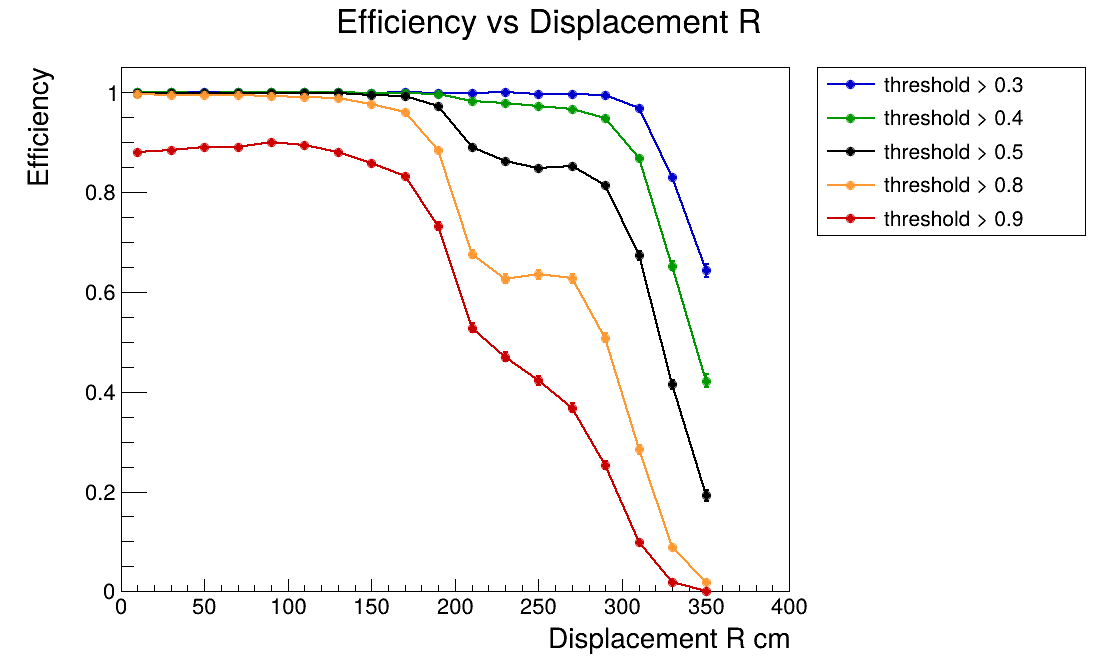
\includegraphics[width=\linewidth]{figures/singlephoton_efficiency_thresholds.png}
    \caption{Efficiency for several shared-energy requirements}
  \end{subfigure}\hfill
  \begin{subfigure}[t]{0.44\textwidth}
    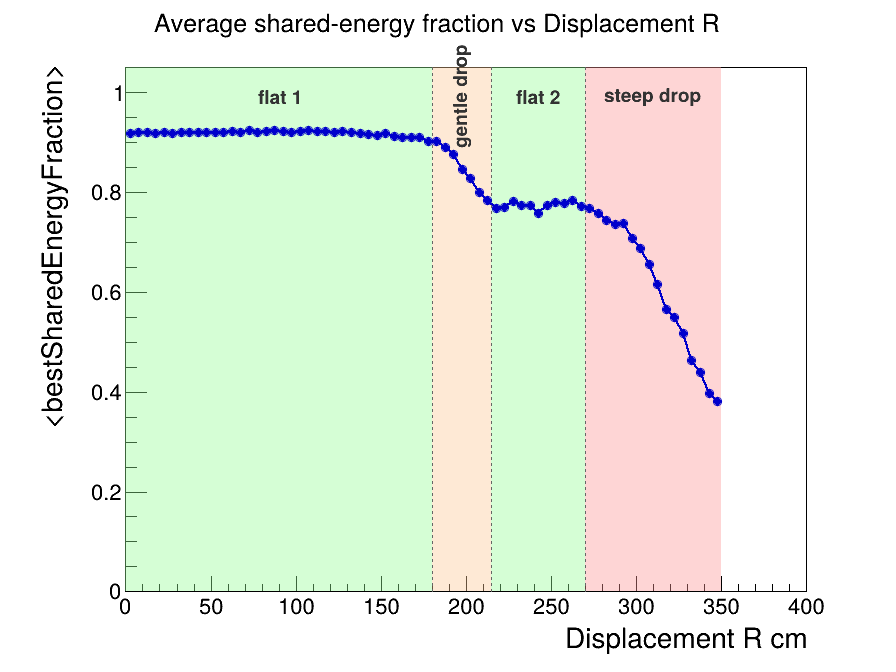
\includegraphics[width=\linewidth]{figures/singlephoton_mean_fraction.png}
    \caption{Mean largest shared-energy fraction}
  \end{subfigure}
  \caption{Single-photon reconstruction without pileup. (a) Efficiency for
  several shared-energy requirements; the black curve is the standard
  $f_{\max}>0.5$. (b) Mean $f_{\max}$, showing the two-stage loss and the
  intermediate plateau. Shaded regions are approximate slope regions.}
  \label{fig:singlephotonperformance}
\end{figure*}

Figure~\ref{fig:singlephotonperformance} shows that the loss is not a smooth
decline. The efficiency is high at small displacement and drops towards
the end, but in between there is a plateau, seen even more sharply in $\langle f_{\max}\rangle$.

This plateau is unexpected: increasing displacement should progressively
violate the pointing assumption, yet reconstruction temporarily stops
deteriorating. The feature persists whatever
shared-energy requirement is used, so it is not a consequence of the $0.5$
efficiency threshold. We will investigate real cause to efficiency loss and plateau.

\subsection{Testing geometric explanations}

\begin{figure}[!tp]
  \centering
  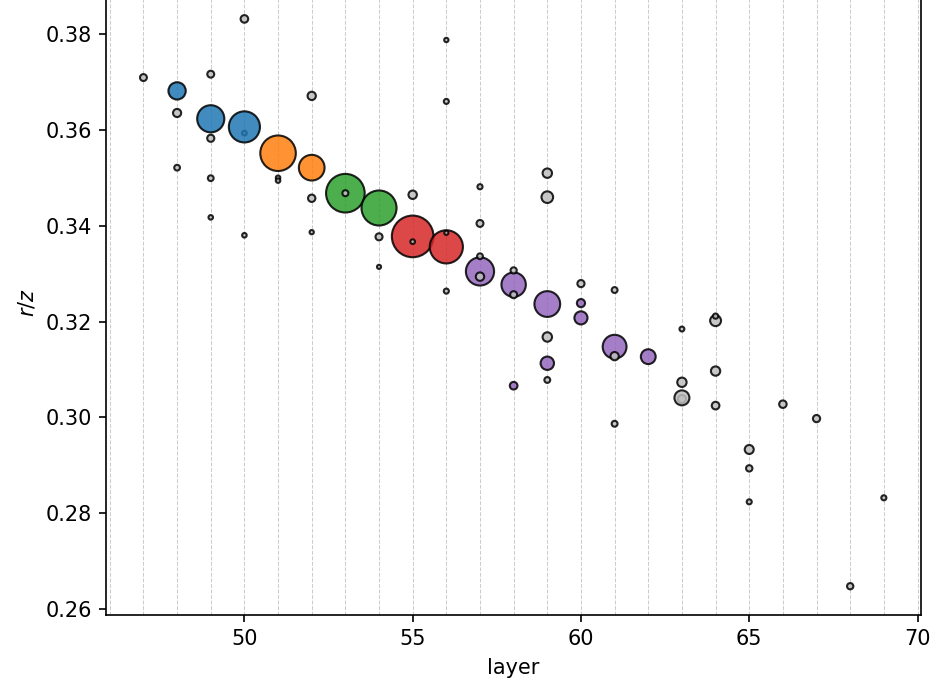
\includegraphics[width=\linewidth]{figures/singlephoton_split_R297_rz.png}
  \caption{A single photon at $\R\simeq\SI{297}{cm}$ split into five
  reconstructed Tracksters, shown as $r/z$ versus layer index. Colour identifies
  the reconstructed Trackster and marker size the energy; grey markers are
  outliers. The layer index follows the TICL convention, in which positive-endcap
  layers are offset to accommodate the negative endcap. $r/z$ is not constant.}
  \label{fig:singlephotonsplit}
\end{figure}

Some explanations can be ruled out quickly. The first is the limited
$(\eta,\phi)$ tile search: a displaced shower does not keep a constant
$(\eta,\phi)$ from layer to layer, so its LayerClusters could drift out of the
search window. But it was not the case, almost every LayerCluster
falls in the same tile as the shower core, at most one tile away, well within
the search reach, so no same-shower neighbour is lost to tiling. The
second explanation is a hidden dependence on trajectory orientation which causes plateau. However, separating photons by
$\Delta\phi(\phi_{\text{origin}}, \phi_{\text{surface}})$ left the plateau
intact, so the mixing of orientations under a
scalar $\R$ does not create the feature either.

\begin{figure}[!tp]
  \centering
  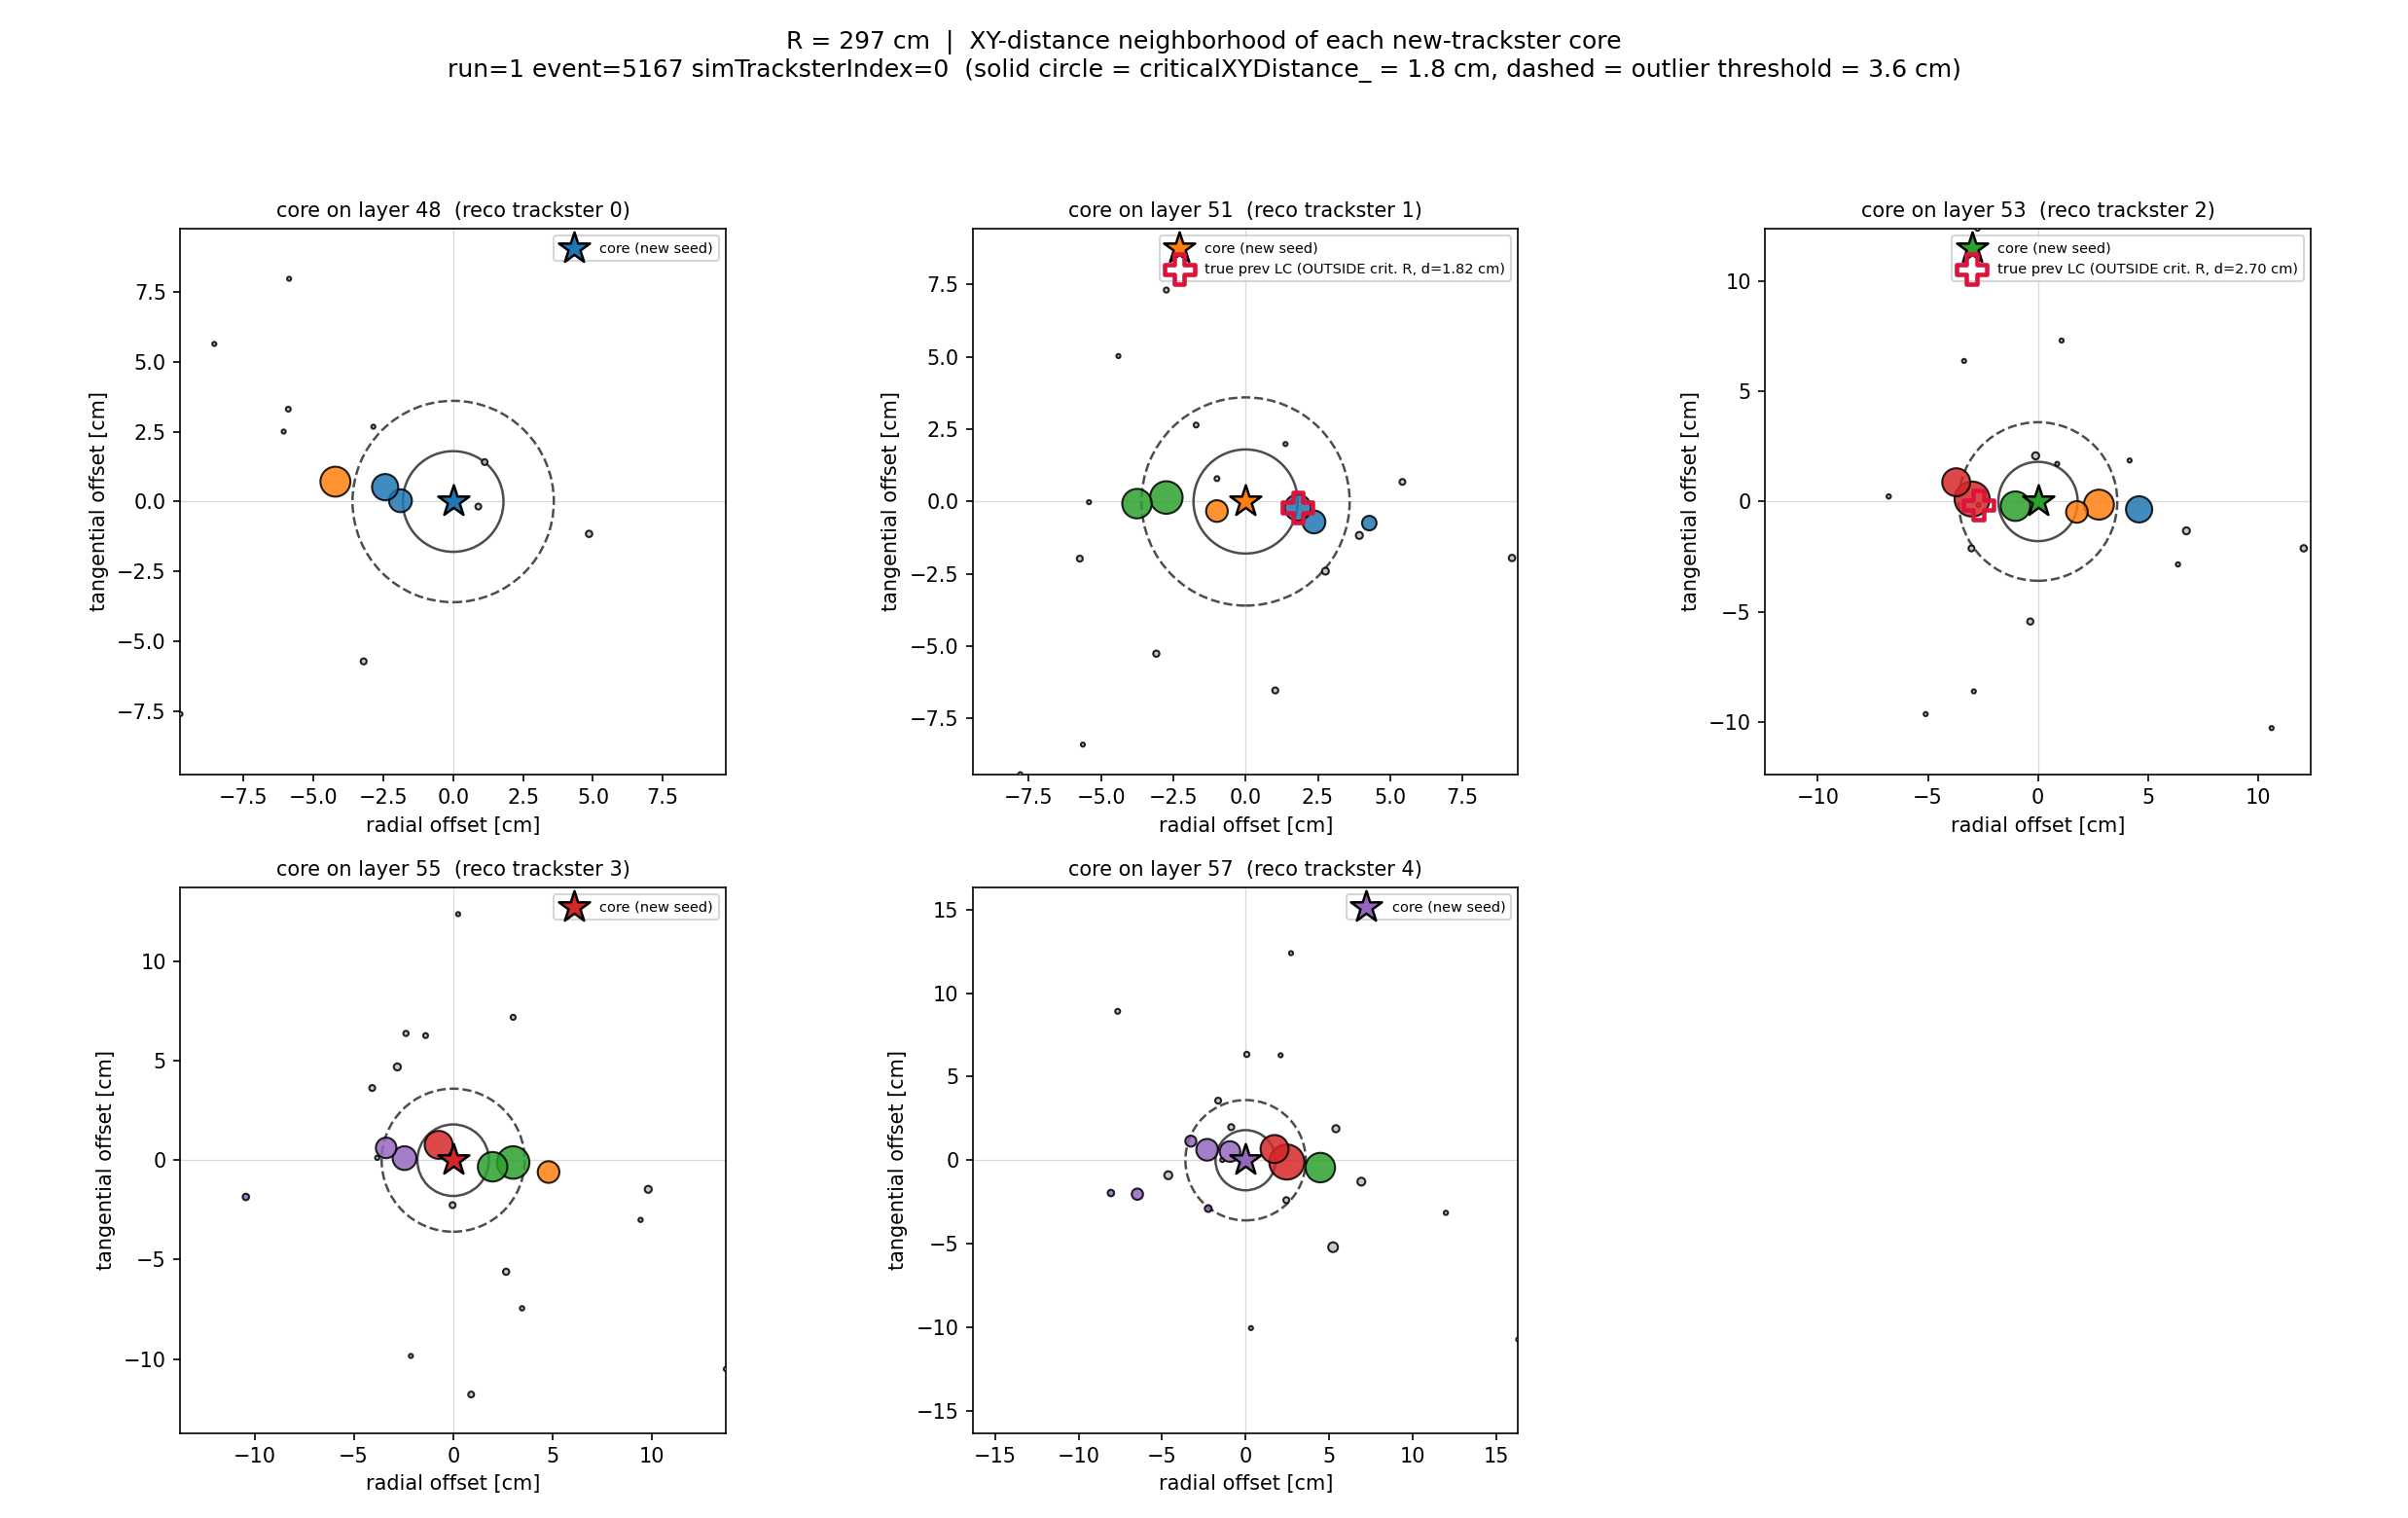
\includegraphics[width=\linewidth,trim=420bp 335bp 417bp 89bp,clip]{figures/singlephoton_neighbourhood_R297.png}
  \caption{A neighbourhood in the full projected coordinates for the
  $\R\simeq\SI{297}{cm}$ event previously shown in
  Fig.~\ref{fig:singlephotonsplit}. The star marks the layer-51 core of a new
  fragment, and circles the \SI{1.8}{cm} and \SI{3.6}{cm} distances.}
  \label{fig:singlephotonneighbourhood}
\end{figure}

\begin{figure*}[!tp]
  \centering
  \begin{subfigure}[t]{0.49\textwidth}
    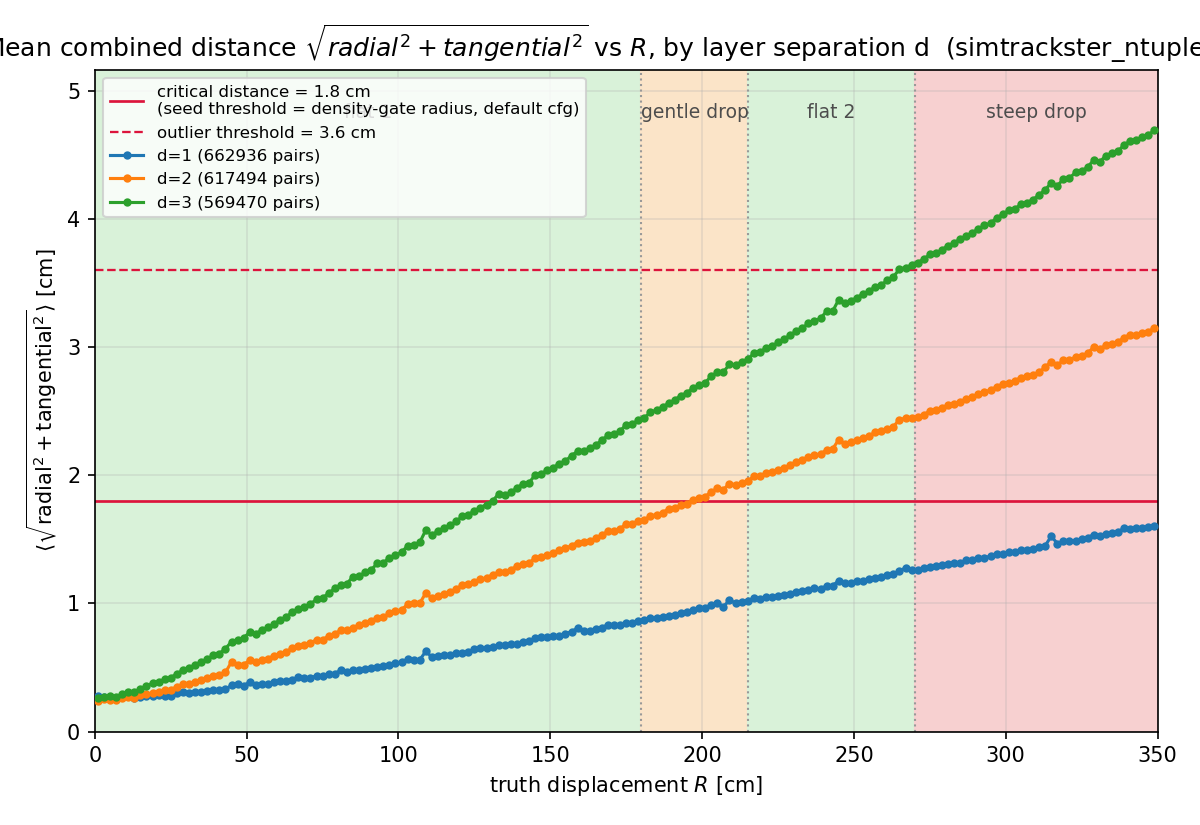
\includegraphics[width=\linewidth,trim=0 0 0 31bp,clip]{figures/singlephoton_pair_distance.png}
    \caption{Full projected distance for core-LC pairs}
    \label{fig:singlephoton-pair-distance}
  \end{subfigure}\hfill
  \begin{subfigure}[t]{0.49\textwidth}
    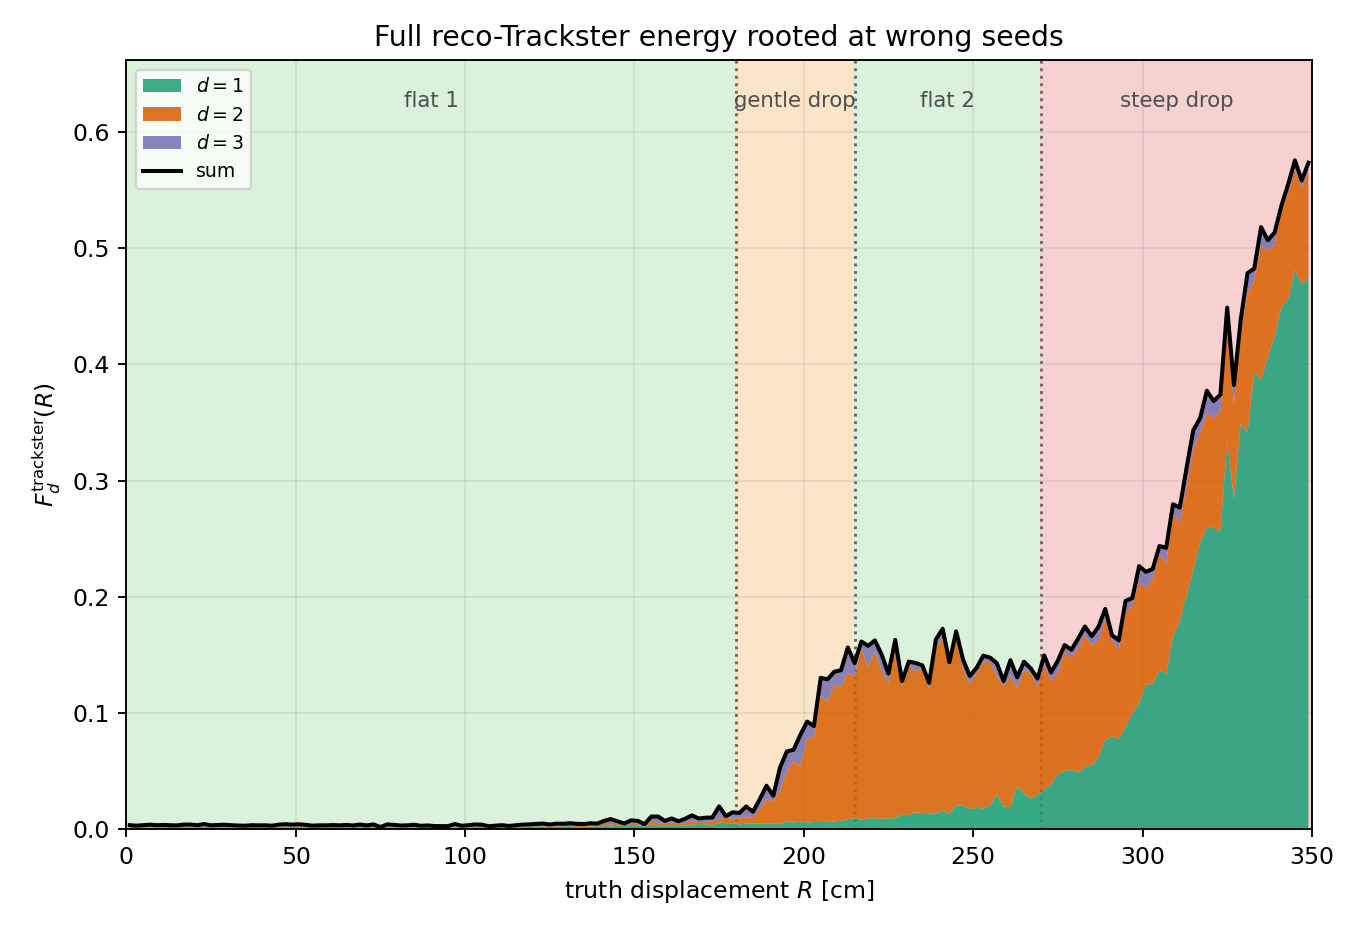
\includegraphics[width=\linewidth]{figures/singlephoton_seed_energy.png}
    \caption{Reconstructed energy in additional seeded fragments}
    \label{fig:singlephoton-seed-energy}
  \end{subfigure}
  \caption{The connection between the geometric threshold and fragmentation.
  (a) Mean full projected distance for LC pairs per $d$. (b) Full reconstructed energy in Tracksters whose
  seed has a higher-density candidate beyond $\SI{1.8}{cm}$, separated by the layer gap $d$ to
  that candidate.}
  \label{fig:singlephotongaps}
\end{figure*}

\subsection{The geometric origin of the growing distance}

The projected distance of Section~\ref{sec:clue3d} suggests a mechanism.
For a straight trajectory, transverse position is
\begin{equation}
  \mathbf{r}(z)=\mathbf{b}+z\mathbf{a},
  \qquad \R=|\mathbf{b}|,
  \label{eq:displacedline}
\end{equation}
where $\mathbf{a}$ is the transverse slope and $\mathbf{b}$ the position at
$z=0$. For a pointing trajectory $\mathbf{b}=0$: both $r/z$ and $\phi$ are
constant along the ideal shower axis. For a displaced trajectory,
$\mathbf{r}(z)/z=\mathbf{a}+\mathbf{b}/z$ changes with depth, as
Fig.~\ref{fig:singlephotonsplit} demonstrates for a real shower.

Projecting a point on layer $j$ to layer $i$ along a ray from the interaction
point gives
\begin{equation}
  \mathbf{r}_{j\to i}
    =\frac{z_i}{z_j}\mathbf{r}(z_j).
\end{equation}
Subtracting this projected position of $j$ from the position of $i$ gives:
\begin{align}
  \Delta\mathbf{r}_{ij}
    &=\mathbf{r}(z_i)-\mathbf{r}_{j\to i}\\
    &=\mathbf{b}\left(1-\frac{z_i}{z_j}\right)
     =\mathbf{b}\frac{z_j-z_i}{z_j}.
  \label{eq:projectionerror}
\end{align}
Thus the exact offset between ideal axis points is
$|\Delta\mathbf{r}_{ij}|=\R|z_j-z_i|/z_j$. For neighbouring layers, and
using the small-angle transverse metric implemented in \cluethreed{},
\begin{equation}
  \boxed{d_{XY}(i,j)\simeq\R\frac{|\Delta z|}{z}.}
  \label{eq:displacedscale}
\end{equation}

Equation~\eqref{eq:displacedscale} explains that distance grows with both
displacement and layer separation even for a perfectly straight photon.
It also gives the approximate scale at which a link exceeds the critical
distance,
\begin{equation}
  \R_{\mathrm{crit}}\simeq\frac{\dm z}{|\Delta z|}.
  \label{eq:criticaldisplacement}
\end{equation}
This supplies a prediction to test against the observed regions.

A first attempt looked promising but proved incomplete. Comparing, for the
most energetic LayerCluster on each layer, the offsets of pairs separated
by $d=1,2,3$ layers, the mean $d=3$ \emph{radial} ($r_i - r_{j \to i}$) offset reaches
$\SI{1.8}{cm}$ near the first decline and the $d=2$ offset near the
second, suggesting that links are lost as displacement
grows. This radial-only picture does not survive once the full projected
distance is used: the azimuthal term of $d_{XY}$ is not negligible, so the
crossings shift.



The local display in Fig.~\ref{fig:singlephotonneighbourhood} shows why the
full distance matters: the same-shower LC from another layer lies
$\SI{1.82}{cm}$ from another seed in projected coordinates, just
outside the critical circle, so two pieces of one continuous shower fall are not satisfying distance criterion.

\begin{figure*}[!tp]
  \centering
  \begin{subfigure}[t]{0.49\textwidth}
    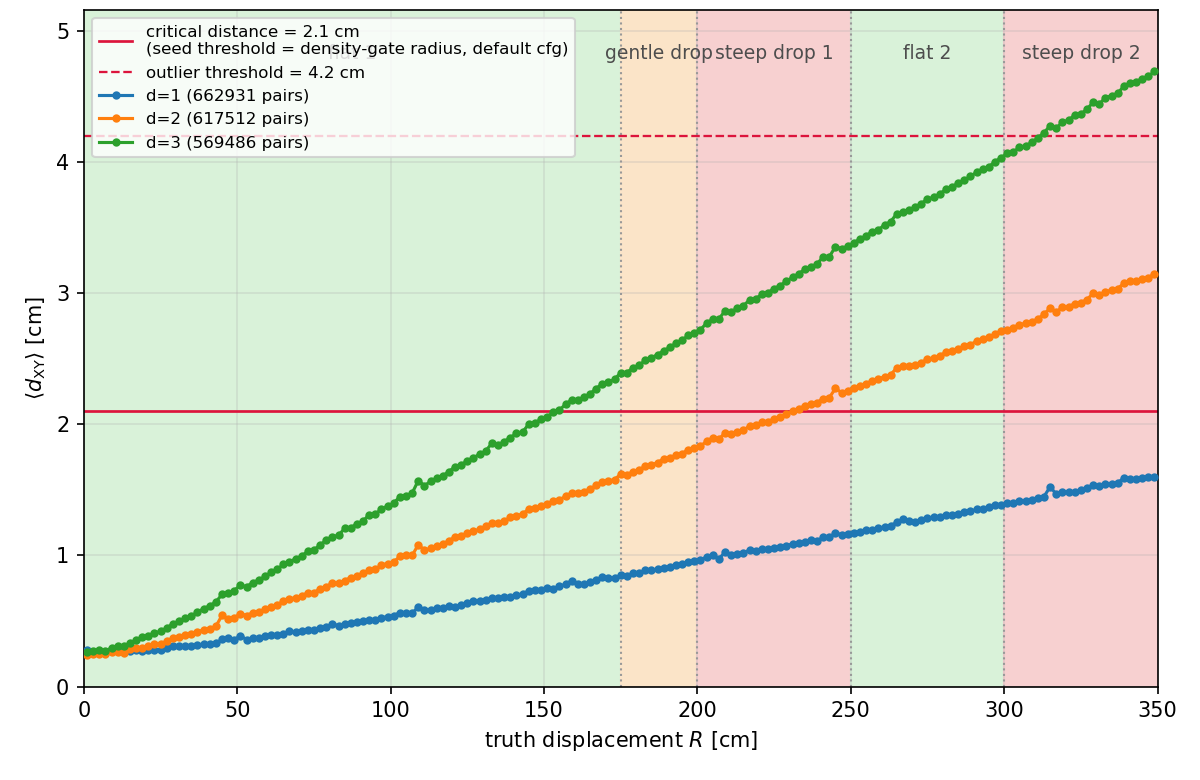
\includegraphics[width=\linewidth]{figures/singlephoton_ablation_pair_distance.png}
    \caption{Full projected distance for core-LC pairs}
  \end{subfigure}\hfill
  \begin{subfigure}[t]{0.49\textwidth}
    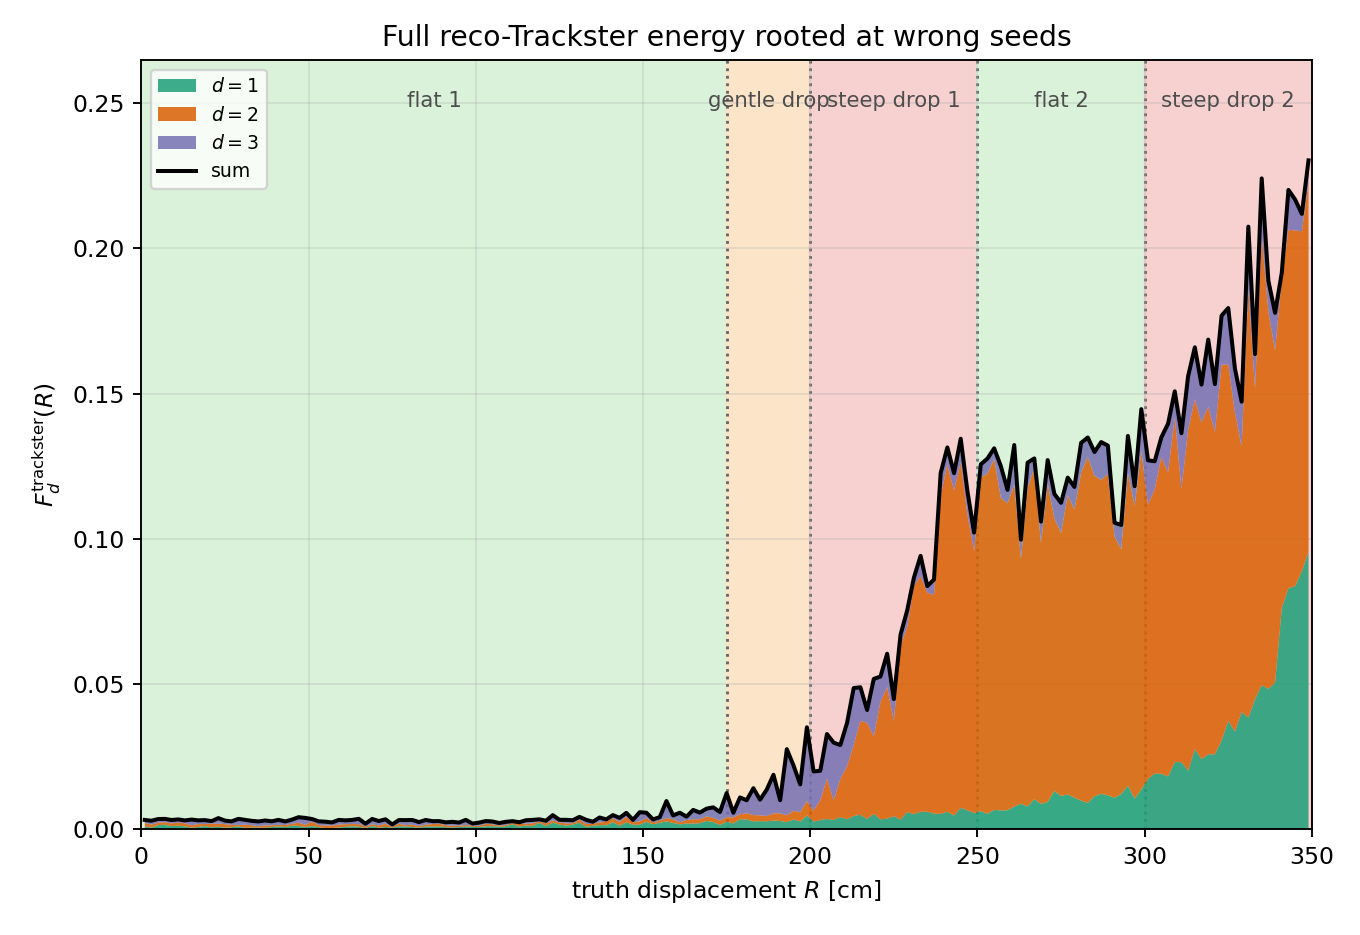
\includegraphics[width=\linewidth]{figures/singlephoton_ablation_seed_energy.png}
    \caption{Reconstructed energy in additional seeded fragments}
  \end{subfigure}
  \caption{The diagnostics of Fig.~\ref{fig:singlephotongaps} for
  $\dm=\SI{2.1}{cm}$.}
  \label{fig:singlephoton-ablation}
\end{figure*}

\subsection{The two-layer transition explains the first loss}



Important insight is shown in Fig.~\ref{fig:singlephoton-pair-distance}.
Near $\R\simeq\SI{200}{cm}$, the mean full projected distance for
$d=2$ pairs crosses $\SI{1.8}{cm}$. At the same time, as shown in
Fig.~\ref{fig:singlephoton-seed-energy}, the energy carried by reco
Tracksters which failed to follow nearestHigher $d=2$ layers away rises sharply. This connects the threshold to the objects that
actually remove energy from the best reconstructed match, which reduces efficiency.

The $d=2$ contribution rises from almost zero to roughly \SI{15}{\%} of the shower energy through the first decline. It then has plateau over
approximately the same displacement range as the plateau in
$\langle f_{\max}\rangle$. The plateau therefore corresponds to a region
where this newly important source of fragmentation has largely stabilized,
before the next one becomes dominant. At larger displacement, the green
$d=1$ contribution rises rapidly and drives the second, stronger loss of
captured energy.

Three-layer pairs cross $\SI{1.8}{cm}$ earliest, but remove little energy, because $d=1,2$ higher-density neighbour can still catch the LayerCluster and prevent a
split. And although the mean one-layer distance stays below $\SI{1.8}{cm}$ for every $R$, individual one-layer links still increasingly exceed it and produce the
observed contribution. This explains the first decline, the plateau and the
second decline.

\subsection{A controlled change of the critical distance}



As a direct test, I reran the HLT reconstruction on the same sample with the
seed distance raised from $\dm=\SI{1.8}{cm}$ to $\SI{2.1}{cm}$, with the density
radius fixed. By Eq.~\eqref{eq:criticaldisplacement} this should push each fragmentation stage to larger $\R$, and it does: the $d=2$ seeded
contribution turns on later, as shown in Fig.~\ref{fig:singlephoton-ablation}. The
degradation moves where the geometry predicts, suggesting
that it is caused by the projected-distance threshold and not just correlated
with displacement.
